\documentclass[10pt]{article}
\usepackage[latin1]{inputenc}
\usepackage{geometry}                % See geometry.pdf to learn the layout options. There are lots.
\geometry{letterpaper}				% Activate for for rotated page geometry
%\geometry{landscape} 
%\usepackage[parfill]{parskip}		% Activate to begin paragraphs with an empty line rather than an indent
\usepackage{graphicx}
\usepackage{epstopdf}
\usepackage{mathptmx}
\usepackage{mathtools}
\usepackage{float}
\usepackage{dblfloatfix}
\usepackage{amsmath}
\usepackage{amsfonts}
\usepackage{amssymb}
\usepackage{multicol}
\usepackage{wrapfig}
\usepackage{amsmath}
\DeclareGraphicsRule{.tif}{png}{.png}{`convert #1 `dirname #1`/`basename #1 .tif`.png}

\begin{document}
\title{Upper Atmosphere and Ionosphere Assignment 3}
\author{Jonathan Nickerson}
\date{February 19, 2012}
\maketitle

\section{Introduction}
In this assignment I continued to improve upon my code by including a zenith angle for the incoming solar flux and allowed it to vary with time. I also built an ionosphere by allowing ions to form in the thermosphere as a function of incoming colar radiation. Since I am short on time this week I will ask for your forgiveness that this writeup isn't going to be quite as stellar as my previous writeups have been. I don't have time to enter the equations and talk about the theory/background. However I think it is a safe bet that you and I both know what equations were used in these calculations: I added the zenith angle, imported the ion cross section data from the text file, calculated production, losses, and number density with the equations you provided in class. This also involved updating the A, B, C, and D values in the tridiagonal matrix. I apologize for having to cut the discussion short this time around. In addition to cutting the writeup short there are also some plots and other parameters I wanted to tweak and play with but unfortunately it will have to wait until next week. For example I only have plots for noon and dawn as of now. My code is set up such that it would take me some time to rerun it and produce more plots for alternative zenith angles. Provided the extra time I would have included plots for the dusk and midnight sectors as well. Below are the plots that were output by my code with some brief explanations.

\begin{figure}[H]
	\centering
		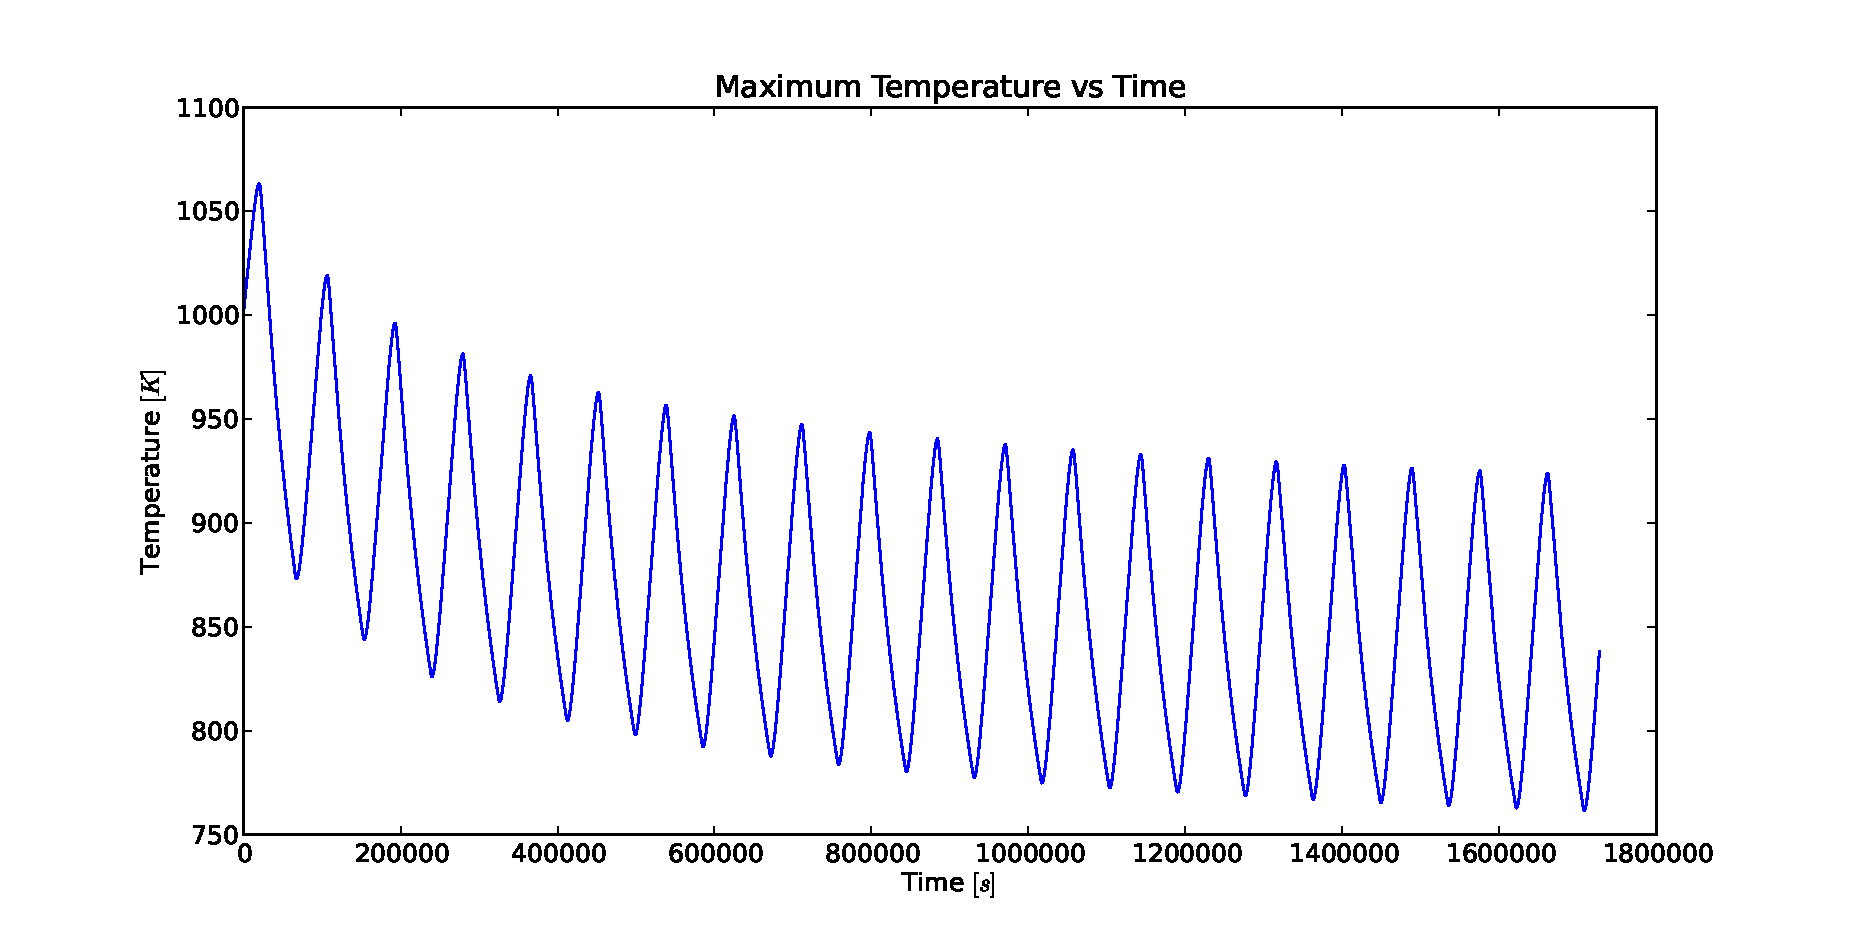
\includegraphics[width=0.99\textwidth]{./noon/A/T_max_vs_time.eps}
	\caption{This is a plot of my maximum temperature vs time. It runs for 20 days. You can see that the general trend is toward an equilibrium temperature range. So on average the temperature has cooled a bit and has begun to level off. After 20 days it is still decreasing slightly so has not yet reached equilibrium. However I did figure that it was close enough by this point. In this plot I have set the zenith angle to begin and end at noon. This decision was completely arbitrary. I also ran the code so that the sun started and set at dawn and not much changed. It can be seen that as the temperature approaches it's equilibrium value it ranges roughly between 750K - 950K over the course of a day. In contrast to assignemnt 2 in which I had calculated a temperature that approached a steady state maximum around 1100K. Compared to real life I believe these new results are a bit on the low side.}
	\label{fig:Tmax}
\end{figure}
\begin{figure}[H]
	\centering
		\includegraphics[width=0.99\textwidth]{./noon/B/Ion_Production_Rate_vs_Altitude_100_800.eps}
	\caption{This is a plot of ion production rate vs altitude for zenith angle $0$ (noon).}
	\label{fig:production1}
\end{figure}
\begin{figure}[H]
	\centering
		\includegraphics[width=0.99\textwidth]{./dawn/B/Ion_Production_Rate_vs_Altitude_100_800.eps}
	\caption{This is a plot of ion production rate vs altitude for zenith angle $-\frac{\pi}{2}$ (dawn). Note how the production decreases by about 2 orders of magnitude when the sun is low in the sky.}
	\label{fig:production2}
\end{figure}
\begin{figure}[H]
	\centering
		\includegraphics[width=0.99\textwidth]{./noon/B/Ion_Number_Density_vs_Altitude_100_800.eps}
	\caption{This is a plot of ion number density vs altitude for zenith angle $0$ (noon). }
	\label{fig:n1}
\end{figure}

\begin{figure}[H]
	\centering
		\includegraphics[width=0.99\textwidth]{./dawn/B/Ion_Number_Density_vs_Altitude_100_800.eps}
	\caption{This is a plot of ion number density vs altitude for zenith angle $-\frac{\pi}{2}$ (dawn).}
	\label{fig:n2}
\end{figure}
\begin{figure}[H]
	\centering
		\includegraphics[width=0.99\textwidth]{./noon/B/Total_Ion_Number_Density_vs_Altitude_100_800.eps}
	\caption{Summing up all of the species and plotting the result gives the total ion number density vs altitude for zenith angle $0$ (noon). Note how the ion production has a large peak in what I might call the F region. What I am uncomfortable with is that the E region isn't really present during the day.}
	\label{fig:tot1}
\end{figure}
\begin{figure}[H]
	\centering
		\includegraphics[width=0.99\textwidth]{./dawn/B/Total_Ion_Number_Density_vs_Altitude_100_800.eps}
	\caption{At zenith angle $-\frac{\pi}{2}$ (dawn) the E region is present. The E region and the F region are clearly distinguishable which is contrary to my understanding of how the ionosphere should be behaving. I will note that the number densities are larger during the day and smaller at dawn which is consistent with what one would expect.}
	\label{fig:tot2}
\end{figure}
\begin{figure}[H]
	\centering
		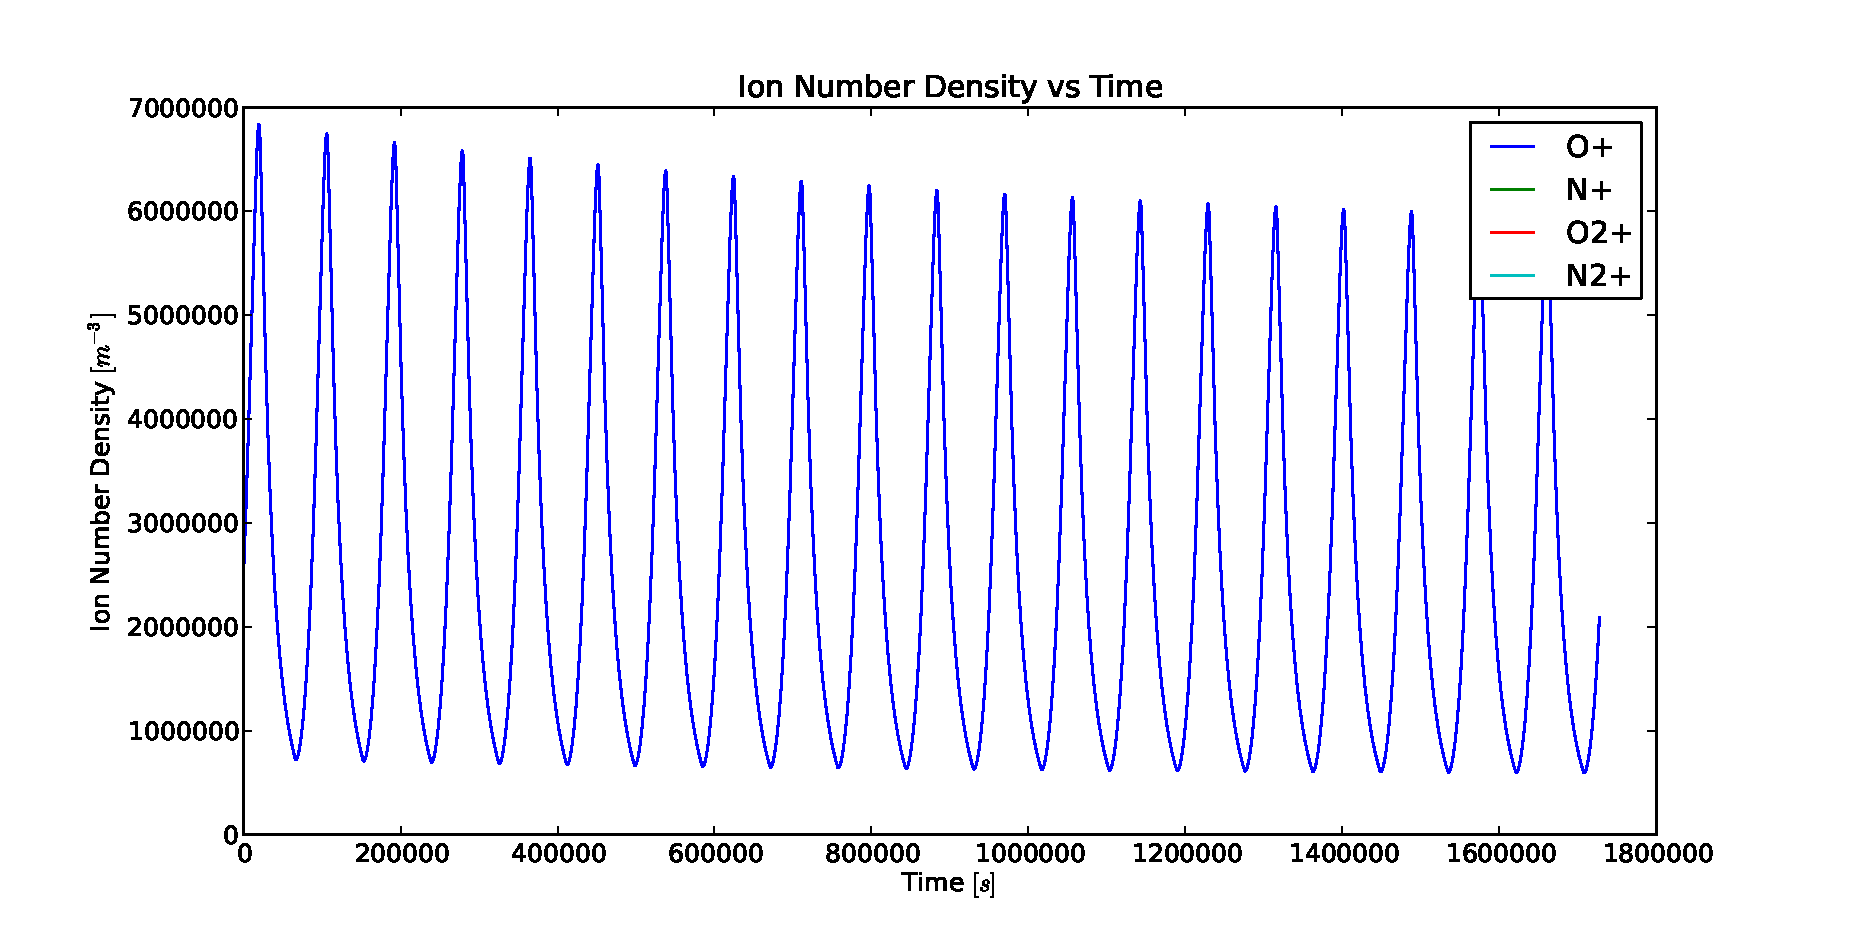
\includegraphics[width=0.99\textwidth]{./noon/B/Ion_Number_Density_vs_time.eps}
	\caption{I calculated the temperature for 20 days first, then ran the program with the ionosphere for an additional 20 days. This final plot is an example of how the number density in the ionosphere changes over the course of 20 days. Since the program is still trying to find its equilibrium temperatuer it is causing the maximum ion number density value to decrease slightly over this timespan. Furthermore it is worth mentioning that this is actually only plotting the value of numberdensity at the very top of the atmosphere. The only species showing up on here is O+ because in this regime O+ is dominating by several orders of magnitude.}
	\label{fig:nvt1}
\end{figure}
\begin{figure}[H]
	\centering
		\includegraphics[width=0.99\textwidth]{./noon/B/Ion_Number_Density_vs_time_log.eps}
	\caption{If we plot this on a logarithmic scale in altitude then we can see the other species change with time as well but then the diurnal variation is harder to distinguish. To keep the diurnal period from getting flattened out too much I made this plot only span the course of one day.}
	\label{fig:nvt1}
\end{figure}






\end{document}
